\chapter{DISSP Design}
\label{ch:system_design}

This chapter introduces the design of the DISSP system, a prototype stream processing system developed to
implement and evaluate the quality-centric data model described in the previous chapter. 
The chapter describes some of the novel features of the design and its implementation.
It shows how the system employs the Source Information Content (\sic) metric to \emph{perform efficiently
under overload} and to \emph{provide feedback} to the user about the achieved quality of processing of
queries.

The system is designed from the ground up to be distributed, allowing the processing of queries to
span multiple compute nodes.
It was particularly targeted at environments with a \emph{constrained amount of resources} that can not
easily be scaled. Examples of such deployment settings include \emph{federated resource
pools} with different authorities administering different processing sites; or \emph{cloud deployments}
in which the resources are rented on demand and it may be more cost effective to reduce the
amount of processing resources voluntarily, trading an acceptable reduction in the correctness of results
for a substantially lower operational costs. 

\emph{Overload} is assumed to be the normal condition of operation for the DISSP system and not a
transient, rare event. 
The \sic values of tuples are used to quantify their importance so that the system can perform an 
\emph{intelligent selection} of which tuples to shed. This allows the creation of \emph{flexible shedding
policies}, as will be shown in the next chapter.
This chapter describes the design choices made to provide a reliable and efficient
processing of queries in such a hostile environment.
It also gives an overview of the different system-level components and their interaction when deploying
and running queries. 

%\pagebreak

%--------------------------------------------------------------------------------------------------------

\section{Design Approach}
\label{sec:design}

%\mnote{4.1 provides the design requirements, tying the overall design and architecture with the needs of
% the model from Chapter 3}

The design of the DISSP prototype system follows the ideas behind the quality-centric data model
from the previous chapter.
The DISSP system places the \sic quality metric at its core and uses it to reason about the
quality of processing achieved by queries.
Every stream is augmented with a \sic value and operators automatically calculate the
new values for their output.
Using \sic values, the system is able to operate under overload, reasoning about the performance of
queries and making intelligent \mbox{load-shedding} decisions.
%When deciding the design of the system, the choice arose about how to implement \emph{tuples} and
%\emph{operators} in an efficient way. The requirements followed in this process were those of
%\emph{performance}, \emph{extensibility} and \emph{efficiency under overload}.

\textbf{Efficiency under overload.}
The system achieves \emph{efficient processing} of tuples and operators. Even though it
is designed to handle resource overload, its occurrence is mitigated as much as possible.
In an overload condition, having to discard some of the input data is always
undesirable to the user. Especially since the system is designed to operate in resource constraint
environments, it should try to maximise its throughput so that the limited available resources
can be fully exploited.
% Overload is considered to be the normal running condition of the system and not a transient condition to
% be overcome. xt
Under an overload condition, the efficiency of the system is inversely proportional to the quantity of
load-shedding so that every increase in system performance leads to a decrease in the
amount of input to be discarded, and thus to an increase of the \sic values of the computed tuples.

\textbf{Meta-data management.}
The DISSP system employs the \sic metric to reason about its performance under overload. The \sic value
of the output tuples delivered to the user is an indicator of the amount of load-shedding
experienced by that query. It provides a mechanism for the system to track the occurrence of failure and
to estimate its impact on the quality of the processed data. It also provides feedback to the user about the
quality of processing achieved by the executed queries.
Every tuple is assigned a \sic value indicating the amount of information that led to its creation.
The mechanism for \sic metric calculations is part of all operators that, after processing, assign a
new \sic value to their output tuples.
Every time a tuple is lost, either due to failure or due to load-shedding, the \sic value of that query
is decreased.

\textbf{Flexible \mbox{load-shedding} policy.}
The use of the \sic values also allows the DISSP system to employ flexible policies when making
load-shedding decisions. When deciding which tuples should be discarded, their \sic values provide
valuable information to the load-shedding component. A perfect value indicates that a tuple was produced
in the absence of failure, while a lower value gives a measure of the amount of lost information.
Using this information, a load-shedder can decide to prioritise some queries over others,
reasoning about the impact that tuple loss would have on their performance. It uses the local
decisions at every processing node to implement a global shedding policy.
Chapter~\ref{ch:load_shedding} focuses on the implementation and testing of a \emph{fair
policy}, which tries to minimise the difference in \sic values experienced by all queries running in
the system.



\begin{comment}
\paragraph{Extensibility} The second main design choice has been \emph{extensibility}. Together with a
set of traditional operators taken from the relational database world, such as Average, Filter, Top-K and so forth, a complete system
should easily allow the implementation of \emph{custom operators}. Even though a great deal of processing
can be carried out with a limited set of operators, many times it is necessary to introduce some new
operators, designed according to the user needs. For instance when dealing with the processing of social
media data, a query could deal with the sentiment analysis of the content, thus requiring the use of
Natural Language Processing operators. The same is true for financial operators implementing proprietary
trading algorithms. For these reasons it was decided to provide the implementation of some generic
operators while allowing the easy implementation of new ones.
\end{comment}


%--------------------------------------------------------------------------------------------------------
\section{Implementing the Model}
% \mnote{4.2 provides a "logical view" of the design, ie these are things that have to be supported that
% clearly derive from the quality-centric data model in Chapter 3; one of of thinking about this is that
% this is the "interface" between Chapter 3 and Chapter 4; some of the material from here could be moved
% to 4.3 to make it shorter...}
This section introduces the basic building blocks of our system. It explains how the theoretical concepts
presented in the description of the data model in Chapter~\ref{ch:data_model} can be actually
implemented. It starts describing the basic concepts related to data, namely \textit{tuples} and
\textit{batches}. After that, it covers \textit{operators}, providing a taxonomy and a description of the
most common ones.
It then describes \textit{queries}, showing how they serve as logical containers for operators and can be
partitioned into smaller entities for distribution. Finally, we introduce the \emph{source time window}
that implements the abstract concept of the \emph{source information tuple set}, which associates \sic
values with input tuples.
\vspace{-10pt}
\paragraph*{Tuples.}
\label{sec:tuples}
Tuples are the simplest unit of information processed by a stream processing system.
As described in Section~\ref{sec:definitions}, they comply with a \textit{schema}, stating the number,
the name and the type of their values.
Values represent the \emph{payload} of a tuple (\ie the data processed by operators in a query).
Every tuple also contains a \emph{timestamp}, an indication of their time of creation.
In our system, this is expressed as POSIX time (\ie the number of seconds that have elapsed since
midnight Universal Time Coordinated (UTC) on January 1, 1970).
A timestamp is typically set externally for \emph{base tuples}, or set by the system when creating
\emph{derived tuples}.\\
Tuples are also associated with an individual \sic value, which expresses the quality of the data carried
in the tuple.
In our implementation, this value is associated with the container batch and not attached to each
individual tuple.
This reduces the overhead of transporting a \texttt{double} value (32 bits) with each tuple, exploiting
our assumption that all tuples within a batch have the same \sic value.
\begin{comment}
\lstset{
  basicstyle=\ttfamily,
  columns=fixed,
  showstringspaces=false,
  commentstyle=\color{white}\upshape
}

\lstdefinelanguage{XML}
{
  morestring=[b]",
  %morestring=[s]{>}{<},
  morecomment=[s]{<?}{?>},
  stringstyle=\color{BrickRed},
  identifierstyle=\color{NavyBlue},
  keywordstyle=\color{ForestGreen}, 
  morekeywords={type,name}% list your attributes here
}
\begin{lstlisting}[language=XML,label=lst:tuplexml,caption=XML description of a Tuple]
	<schema name="simpleSchemaONE">
	    <field type="long"   name="ts"  />
	    <field type="double" name="idx" />
	    <field type="double" name="tmp" />  
	</schema>
\end{lstlisting}


As described in Section~\ref{sec:templates}, Tuples are implemented using a template file. One parent
class called ``Tuple'' is provided, containing the basic logic common to all tuples, and every other
tuple class derive from this. In the XML query description, the user specifies a schema and a name for
the tuples that will be used by the query and the system creates a new tuple class, with the name and
fields required. A generic tuple \texttt{.template} file is filled, substituting some placeholders with
the provided data, producing the \texttt{.java} source file of the new tuple class.

Listing~\ref{lst:tuplexml} shows the XML description of a Tuple object with 3 fields: one \texttt{long}
for the timestamp named \textit{ts}, and two \texttt{double}, one with a numerical identifier \textit{idx}
and the other carrying a temperature reading \textit{tmp}. These values will be inserted in the tuple
.template in correspondance with the ``\texttt{\$FIELD}'' placeholder, transforming it into a complete
.java source file. The compiled object will contain 3 public fields with the type and name specified in
 the XML listing.
\end{comment}
\vspace{-10pt}
\paragraph*{Batches.}
\label{sec:batches}
Batches are logical groups of tuples with the same \sic value. Instead of associating an individual
metadata value with each tuple, the system uses batches as containers with a single \sic value, which is
considered valid for all the tuples contained in that batch.\\
Batches are the input and output units of operators. The output of an operator may be composed of
several tuples, which are encapsulated within a batch. The operator calculates a \sic value for all
tuples in the batch based on the \sic values of the input batches and its processing semantics.
The newly produced batch is delivered as input to another operator or is returned as a result to the
user.

Batches are an implementation of the CQL concept of a \textit{relation}, as described in
Section~\ref{sec:cql}.
They represent a finite snapshot of a stream, which allows operators to process a potentially infinite
continuous stream of tuples in consecutive, discrete steps. By using batches, the DISSP system does not
need to use \textit{stream-to-relation} or \textit{relation-to-stream} operators because batches provide
a unified input/output unit for operators. A stream becomes an abstract entity as a potentially infinite set of
batches, while batches serve as the actual units of information in the system.
In our system, batches are simple objects that contain a list of tuples, a \sic value and some additional
metadata. 
% They also contain the logic for converting to and from their network representation.
% --------------------------------   OPERATORS 	--------------------------------	
\paragraph*{Operators.}
\label{sec:operators}
Operators are the basic unit of computation in a stream processing system. They implement a
\textit{function} that transforms one or more input batches to one output batch. A set of operators
linked together in a directed acyclic graph is referred to as a \textit{query}.

Operators can be classified as \textit{blocking} or \textit{non-blocking} based on their behaviour when
handling input data. Many operators can be configured to work in either mode. 
\textit{Blocking operators} need at least one input batch on every input channel before they can
produce an output, while \textit{non-blocking operators} execute every time a new batch of tuples is
delivered on either input. 
% The system implements the logic described in Section~\ref{sec:definitions}.

\begin{figure}
	\centering
	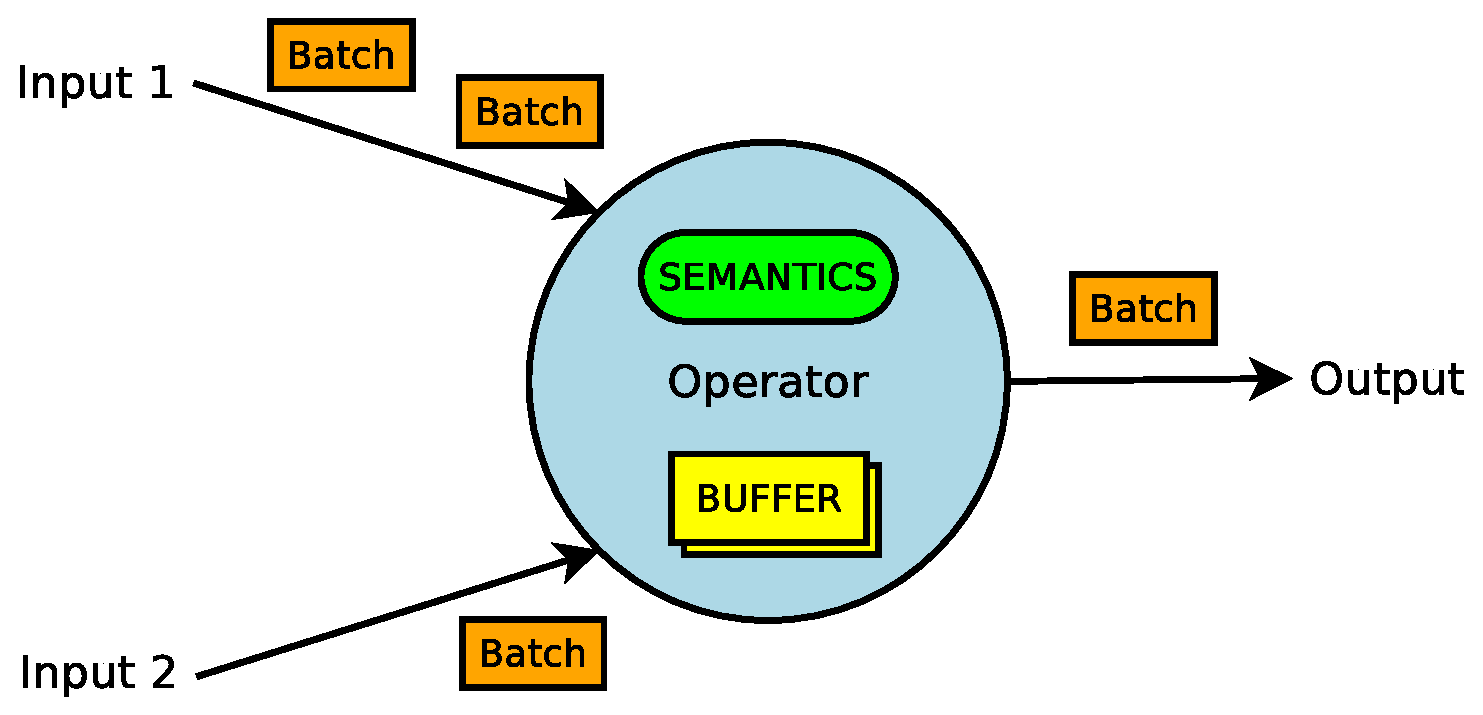
\includegraphics[width=0.6\textwidth]{img/tesi/operator2.eps} 
	\caption{A generic operator with its internal structure shown.}
	\label{fig:op2}
\end{figure}    			

Figure~\ref{fig:op2} shows the internal structure of an operator with its two main components: the
\textit{buffer pool} and the \textit{semantics module}. Every operator is equipped with a pool of
internal buffers, one for each input channel. These are used to stage tuples before they are processed. Every
time an operator triggers for execution, it first moves one or more batches of tuples into the
corresponding buffer within the pool.
A buffer may still contain tuples from the previous execution cycle. In this case,
the new batch is merged with the leftover tuples.

After the input data was staged, the operator executes the logic contained in the \textit{semantics 
module}. This is what characterises an operator by defining its processing logic.
From an implementation point of view, an operator is an abstract class with an unimplemented
\texttt{execute()} function. A concrete operator class has to provide the code for this function. 
Once an operator finished processing, this function returns a batch of tuples that are delivered as its
output.
% From the standpoint of a user, implementing a new custom operator boils down to the definition of
% a new java class, extending either the \textit{BlockingOperator} or the \textit{NonBlockingOperator} class,
% which implements the \texttt{execute()} method. To make this class generic it is then necessary to
% convert it into a \textit{template} file. This is done by replacing some fields with a generic placeholder
% which will then be specified in the XML description of this operator.
\begin{comment}
Listing~\ref{lst:opxml} shows the XML description of an \textit{Average} operator. In the first line the
operator is characterized as being an instance of class ``Average'', described in the correspondent
.template file, and it is given the name of ``MyAvgCpu'. Then there is the declaration of a \textit{next}
operator, this means that this is not a terminal operator and thus its output should be delivered to a
single local operator named ``MyOutput''. Next are 3 parameter definitions, in the form $\langle name,
value \rangle$. The system will look for the ``\$NAME'' placeholder and will replace it with the string
given by ``value''. Once the substitution has taken place, the .template file becomes a complete .java
source file and is then compiled by the \textit{CharSequenceCompiler}.
		 
\lstset{
  basicstyle=\ttfamily,
  columns=fixed,olding,
  showstringspaces=false,
  commentstyle=\color{white}\upshape
}

\lstdefinelanguage{XML}
{
  morestring=[b]",
  %morestring=[s]{>}{<},
  morecomment=[s]{<?}{?>},
  stringstyle=\color{BrickRed},
  identifierstyle=\color{NavyBlue},
  keywordstyle=\color{ForestGreen}, 
  morekeywords={type,name}% list your attributes here
}
\noindent\begin{minipage}{\textwidth}
\begin{lstlisting}[language=XML,label=lst:opxml,caption=XML description of an Average operator]
	<operator name="MyAvgCpu" type="Average">
	    <next name="MyOutput"/>
	    <parameter name="tuple"    value="simpleSchemaONE" />
	    <parameter name="field"    value="cpu"/>
	    <parameter name="groupby"  value="idx"/>
	<operator>
\end{lstlisting}
\end{minipage}

In the next sections there will be an overview of the main classes of operators provided by the DISSP
prototype. \textit{Window Operators} provide transformations over window sizes, holding the input of an
operator until a certain condition is reached. \textit{I/O Operators} are the gateways to the system, in
input they provide the conversion from external to system tuple representation, in output they deliver
the query results to the user. \textit{Network Operators} allow the inter node communication, so that a
query can be partitioned and distributed onto several nodes. Finally there will be a list of the main
\textit{Data Manipulation Operators}, these are the ones actually performing the processing on the data,
and are equivalent to the \textit{relation-to-relation} operators in CQL.

\mnote{Where should I place the operator list? Here seems a bit dispersive}

\subsubsection*{Window Operators}
\label{sec:window-op}
Window Operators provide a way of regrouping tuples, changing the size of their container batches and are
equivalent to the \emph{stream-to-relation} operators in CQL. 
In CQL a stream is a continuous entity and needs to be broken down into a series of relations through a
\emph{stream-to-relation} operator before operators can process it. In our system a stream is a purely 
abstract entity, since batches already are series of tuple snapshots but window operators are still used
to group the input of an operators, so that every new input batch contains tuples with a precise
semantic. The regrouping of tuples can be done according to their \emph{timestamp}, according to the
values of a \emph{field}, or according to their \emph{position} in the stream.

\paragraph{Sliding Windows}


\paragraph{Time Window}
A \emph{Time Window} defines a temporal interval and produces an output batch containing all the tuples
received during the interval. For instance a time window of interval ``1 minute'' outputs a batch of
tuples every minute, containing all tuples received in the previous 60 seconds. The incoming tuples
accumulate in the internal buffers until the current time interval is over, then they are grouped into a
new batch that is sent in output and a new time interval begins. 

\paragraph{Field Window}

\paragraph{Count Window}
A \emph{Count Window} defines a new output batch composed by an exact number of tuples. For instance a
count window of size N always produces batches of N tuples in output. If an input batch contains M
tuples, with M greater than N, it gets broken down into a series of batches of size N, until the
remaining tuples are less than N. These remainder tuples sit in the internal operator buffer until they
are merged with a new incoming batch. When a new batch arrives it is merged with the tuples still present
into the internal buffer from the previous execution and, if their total amount is greater than N, a new
output batch is produced.   

			
	
	
		\subsubsection*{I/O Operators}
		\label{sec:input-output}
			\paragraph{Source Input Device}
			\paragraph{Output Device}
		
		\subsubsection*{Network Operators}
		\label{sec:network-op}	
			\paragraph{Remote Sender}
			\paragraph{Remote Receiver}
		
		\subsubsection*{Data Manipulation Operators}
		\label{sec:data-op}				
			\paragraph{Filter}
			\paragraph{Average}
			\paragraph{Covariance}
			\paragraph{Join}
			\paragraph{TopK}
			\paragraph{Union}
			\paragraph{Min}
			\paragraph{Max}
\end{comment}
% --------------------------------   QUERIES 	--------------------------------		
\paragraph*{Queries.}
\label{sec:queries}

A query logically groups operators that cooperate in the same processing task.
In our design, a query is organised according to the \emph{boxes-and-arrows} model. 
A user submits a query specification containing the list of operators and the connections among them. 
Within a query, operators are organised in a directed acyclic graph. 

A query always starts with one or more \emph{input operators}, which transform the
incoming data streams into the DISSP system format. They thus act as a gateway, allowing external input
generators, such as a sensor network, to connect to the system and make their data available for
processing.\\
In addition, there are a number of \emph{data manipulation operators} that take data items and
process them according to the query semantics. After a final result was obtained, it is delivered to
the user through an \emph{output operator}. 
%The different classes of operators are further described in Section~\ref{sec:operators}.

As described in Section~\ref{sec:fan-in}, the graph of a query have different shapes. Fan-in queries
include a single output operator, while fan-out queries permit for more than one final result and thus
have multiple terminal operators.

\paragraph*{Subqueries.}
Queries may become too computationally expensive to execute completely on a single processing node. 
To avoid overload, the query graph can be split into a number of partitions, which are referred to as
\emph{subqueries}.
The partitioning of a query can follow different strategies, \eg grouping operators according to
equal computational costs or distributing the same subquery for parallel processing. The different query
partitioning schemes are described in Section~\ref{sec:qpart}.

Subqueries are deployed onto several processing nodes. For each query in the system, there is
a \emph{coordinator} that is in charge of the partitioning, deployment and management of the query. It
uses a system of \emph{command messages} to obtain a set of suitable nodes for deployment and to install
the subqueries on the processing nodes. After the query was deployed, data can start flowing
through the input operators and the processing begins.
% --------------------------------   QUERIES 	--------------------------------	
\paragraph*{Source Time Window.}
\label{sec:stw}
Section~\ref{sec:sits} introduced the concept of the \emph{source information tuple set}: the set of
input tuples from which a final result is generated. In the absence of failure, the final \sic value of a
tuple is the sum of the \sic values of all tuples contained in the corresponding source information tuple
set.
According to the model definitions stated in Chapter~\ref{ch:data_model}, every source contributes a
total unnormalised \sic value of $1$ to all result tuples. 
% Every tuple contributing to
% a result passes through an \emph{input operator} and is assigned a \sic value of $1$ divided by the total
% number of participating tuples.

To implement this part of the data model in practice, it would be necessary to know in advance which
tuples will contribute to the creation of a future result. Since the result has not yet been created,
however, it is infeasible to identify the source information tuple set and thus to define it accurately
due to the time delays during query processing caused by processing delays, variable-sized time windows,
etc.
To address this challenge, we consider an approximation: a source information tuple set that includes all
source tuples generated by sources during a predefined time period, referred to as the \emph{source time window (STW)}.

The length of a STW is chosen so that it is always longer than the greatest possible end-to-end query
processing delay.
In this way, the STW contains all tuples that can possibly contribute to the generation of future results.
In practice, a STW may include source tuples that generate multiple different result tuples, or
belong to different source information tuple sets.
Therefore, we apply the same concept of the STW to the result streams as well: the result \sic value of a
query is the aggregate \sic value of all result tuples generated during the same STW.
In order to capture the continuous nature of processing in data streaming, we treat the STW as a
sliding window with a small slide compared to its size.

%%
By using the STW, we no longer require the precise definition of the source information tuple set
$\mathcal{T}^{S}$ and result tuple set $\mathcal{T}^{R}$. Rather, we can use two new sets:
$\mathcal{T}^{S}_{STW}$, which is the set of input tuples belonging to a source time window, and
$\mathcal{T}^{R}_{STW}$, which is the set of output tuples belonging to the corresponding window on
the result streams. 

Using these new tuple sets, the definition of the result \sic value of a query becomes:
\begin{align} 
		\sic_Q = \sum_{t_R \in \mathcal{T}^R_{STW}} t_{R}^{SIC} = \sum_{t_{src} \in \mathcal{T}^{S}_{STW}}
		t_{src}^{SIC},
\end{align}

This definition states that, in the absence of failure, the sum of all \sic values of tuples in a source
time window is equal to the sum of all \sic values of the tuples present in the corresponding window on
the result streams.
% 
% %%
% 
% 
% The \sic value of a derived tuple $t$ processed by operator $o$, \ie $t \in \mathcal{T}_{out}^{o}$, is: 
% % \begin{align} 
% % 	t_{SIC} = \displaystyle\sum_{t \in \mathcal{T}_{in}^{o}}{t_{SIC}} \cdot
% % 	\frac{1}{|\mathcal{T}_{out}^{o}|}
% % \end{align}
% \begin{align} 
% 	t_{SIC} =
% 	\frac{1}{|\mathcal{T}_{out}^{o}|} \cdot \displaystyle\sum_{t \in \mathcal{T}_{in}^{o}}{t_{SIC}} 
% \end{align}
% By using the STW, we no longer require the precise definition of the $\mathcal{T}_{in}^{o}$ and
% $\mathcal{T}_{out}^{o}$ sets. Rather, we can use two new sets for each operator $o$:
% $\mathcal{T}_{in}^{o\prime}$ is formed by the window operator before $o$ and $\mathcal{T}_{out}^{o\prime}$
% depends on the semantics of $o$. Note that $\mathcal{T}_{in}^{o\prime}$ and $\mathcal{T}_{out}^{o\prime}$
% may not contain the correct set of tuples to produce a result tuple. However, we ensure that the
% calculation of the result tuples is correct according to the data model definition of \sic by applying the same STW at the result stream.
% %Section~\ref{sec:eval_stw} will evaluate this approach, showing that the STW correctly captures perfect
% %processing with a negligible error.


%--------------------------------------------------------------------------------------------------------

\section{DISSP Architecture} 
% 
% \mnote{4.3 describes the overall architecture, ie it provides the components that will realise the
% logical design from 4.2; as you say, this section should be ls onger than 4.2}
% 
This section describes the overall architecture of the DISSP system.
First, it presents the \emph{high-level components} of a system deployment. DISSP is a distributed
system that is designed to be deployed on a large number of nodes. Every system-wide component that
takes part in the processing of a query will be described, emphasising its role within the
system.

After that, we present the \emph{node architecture}, focusing on the internal operations of a
DISSP node. The different components of a processing node are examined, providing details of some of the
implementation choices and the reasoning behind them. In particular, we describe the
network layer that handles inter-node communication, the operator runner that realises the query
semantics, the load-shedder used to manage overload and the statistics manager that collects
information on the system status.
% 
% When a batch of tuples is received by the node is delivered to the right subqueries, it gets
% processed and finally it is forwarded to the next node to continue processing. A description of these
% steps and about the internal components needed will end the section.
% 
% \todo{WRITE LONGER INTRO!!}

%\clearpage
%
% % -------------------   TEMPLATES   --------------------
% \subsection{Compiled Operators and Tuples}
% \label{sec:templates}
% 
% \mnote{Should this go here? Otherwise, where?}
% 
% In our system tuples and operators are implemented as \emph{compiled POJO objects}. This choice was made
% taking performance into consideration, since other options, based for instance on \emph{reflection}, were considered too
% slow and cause of a potential performance bottleneck. To instantiate a custom tuple or operator object,
% based on the query requirements, a text \textit{template} is completed with the information contained in the XML file
% describing the query producing a new .java file, which is then compiled to bytecode by a run-time compiler. 
% 
% \paragraph{XML Query Representation} Queries are submitted to the system using and XML representation. An
% XML query file contains the complete description of the query. It specifies what kind of tuples will be
% processed, providing a description of the \emph{tuple schemas} so that operators are aware of the
% number, type and name of the fields contained in the tuples they process. It also contains the list of operators
% implementing the query semantic. Every operator is represented by an XML block, containing its
% description. Every operator needs to be specialised before it can be used within a query. A generic
% implementation is provided in a \emph{template file}, which acts as a blueprint for the operator, which
% is then finalised with the data included in the XML block, allowing the correct instantiation of the
% operator.
% The information needed to complete an operator templates includes its \emph{name, parameters} and an indication about its \emph{following operator}. Every operator either declares itself as a
% \emph{terminal} operator, by declaring no downstream operators, or as an \emph{intermediate} operator by
% declaring that its output should be fed in input to another operator. This allows the system to
% reconstruct the complete query graph. 
% The information contained in the XML representation is used to generate the complete .java files
% describing theon customised tuples and operator that will be used in the query. This can then be compiled
% and instantiated so that the query can begin processing. 
% 
% \paragraph{Templates} are semi-complete \textrm{.java} files, representing the skeleton of a class. 
% They are used for the efficient instantiation of customised \textit{tuples} and \textit{operators}.
% All tuples share some common characteristics but are differentiated by the number of fields, their names
% and types. The same is true for all operators belonging to the same type. For instance Average operators
% are all equals when it comes to the processing semantic but they differ about the name and type of the
% field to be averaged. So a generic blueprint for these object comes from the generalisation of a specific
% instance, where specific names and types are replaced by some place text tokens called \emph{place
% holders}. Using the information contained in their XML description it is possible to substitute these
% place holders with the correct details, transforming a template into a complete \textrm{.java} ready for
% compilation.
% Place holders are all capital keywords preceded by a dollar sign, in the
% form ``\texttt{\$PLACEHOLDER}''. They are meant to be completed using the information provided in the XML
% file describing the query and the compiled into actual POJO objects with the desired characteristics. For
% this transformation the system employs a \textit{CharSequenceCompiler}, which takes in input a string
% containing the content of a completed \textrm{.template} file and produces an instance of the customised
% object.
% This allows the system to operate always on compiled bytecode, granting the maximum performance of
% execution together with the flexibility of working with customised versions of tuples and operators
% tailored to the specific query requirements.
% \lstset{
%   basicstyle=\ttfamily,
%   columns=fixed,
%   showstringspaces=false,
%   commentstyle=\color{white}\upshape
% }
% 
% \lstdefinelanguage{XML}
% {
%   morestring=[b]",
%   %morestring=[s]{>}{<},
%   morecomment=[s]{<?}{?>},
%   stringstyle=\color{BrickRed},
%   identifierstyle=\color{NavyBlue},
%   keywordstyle=\color{ForestGreen}, 
%   morekeywords={type,name}% list your attributes here
% }
% \noindent\begin{minipage}{\textwidth}
% \begin{lstlisting}[language=XML,label=lst:opxml,caption=XML description of an Average operator]
% 	<operator name="MyAvgCpu" type="Average">
% 	    <next name="MyOutput"/>
% 	    <parameter name="tuple"    value="simpleSchemaONE" />
% 	    <parameter name="field"    value="cpu"/>
% 	    <parameter name="groupby"  value="idx"/>
% 	<operator>
% \end{lstlisting}
% \end{minipage}
% 
% \exblock{Listing~\ref{lst:opxml} shows the XML description of an \emph{Average} operator. In the first
% line the operator is characterized as being an instance of class ``Average'', described in the correspondant
% .template file, and it is given the name of ``MyAvgCpu'. Then there is the declaration of a \emph{next}
% operator, this means that this is not a terminal operator and thus its output should be delivered to a
% single local operator named ``MyOutput''. Next are 3 parameter definitions, in the form $\langle name,
% value \rangle$. The system will look for the ``\$NAME'' placeholder and will replace it with the string
% given by ``value''. Once the substitution has taken place, the .template file becomes a complete .java
% source file and is then compiled by the \emph{CharSequenceCompiler}.}
% 	
% 
% --------------------   SYSTEM   --------------------
\vspace{-10pt}
\subsection{System-level Components}

\begin{figure}[b!]
	\centering
		\includegraphics[width=0.6\textwidth]{img/tesi/system_design} 
	\caption{A system level overview of the components in DISSP prototype. }
	\label{fig:sys}
\end{figure}
This section presents the system-level components in the DISSP prototype stream processing system. 
The most important component of all is the \emph{processing node}, a dedicated machine used for the
processing of queries. One or more processing nodes constitute the resource pool onto which all queries
are deployed. Since a query is usually divided into subqueries that are hosted on different processing
nodes, a \emph{coordinator} is deployed for each query. It is hosted on a separate machine and
is in charge of monitoring the status of the query (\ie detecting failed nodes and gathering statistics
about the query performance in terms of achieved quality of processing). \\
A number of data \emph{sources} provide input to the processing nodes. A system-wide \emph{oracle} is
used to obtain a global view of the system. It is aware of all queries and their performance, allowing
to monitor the behaviour of the system as a whole, and is used during query deployment by the
coordinator to provide a list of processing nodes suitable for the deployment of a new query. Finally,
there is also a \emph{submitter}, which provides the user interface to submit one or more queries
for execution. 

Figure~\ref{fig:sys} provides a high-level overview of the DISSP system. Many \emph{processing
nodes} can be deployed in a cloud environment, while some \emph{sources} provide the input data to be
processed.
Queries are deployed through a \emph{submitter}, each having an associated \emph{coordinator} in charge
of its management. An \emph{oracle} oversees the processing of all queries. It gathers information
about their status and performance and also provides the set of nodes onto which new queries
should be deployed.
\vspace{-10pt}
\paragraph*{Processing Node.}
The \emph{processing node} is the component in charge of the execution of operators. It receives tuples through
a network connection. Tuples are converted from their serialised network representation into
concrete instances.
Tuples are then sent to the graph of operators in charge of their processing. After processing by one
node, tuples are sent to the next node to be further processed by the next subquery or are sent to the
output if there is no more processing to be done. Every \emph{processing node} periodically reports to the query \emph{coordinator} about the performance
achieved in terms of quality of processing and to the \emph{oracle} about its throughput and load
condition.
All \emph{processing nodes} are also in charge of performing \emph{load-shedding}, whenever an overload
condition arises. They then make local decisions about which input tuples should be discarded in order to
reduce load. A \mbox{load-shedding} policy designed to achieve \emph{fairness} among all queries running
in the system is the topic of Chapter~\ref{ch:load_shedding}.
% A more detailed description about the internal components and functioning of a \emph{processing node} will be
% provided in Section~\ref{sec:node-arch}.

% \exblock{
% \texttt{java qp.misc.DisspNode <nodeIP> <nodePORT> <oracleIP>}
% 
% This command starts a Processing Node at $\langle nodeIP\rangle$ on port $\langle nodePORT\rangle$.
% The location of the oracle is also passed to the processing node so that it can signal its existence
% and report about its status. After initialisation the processing node remains dormient, until a
% coordinator selects it as a host for the execution of a subquery. 
% } 

\paragraph*{Submitter.} Queries are deployed in the system through the invocation of a
\emph{submitter}.  It receives as input an XML file with the query specifications, including the
\emph{tuple schemas} to be used and the \emph{list of operators}, specifying their type, name, parameters
and connections.
Based on this query description, the \emph{submitter} compiles the individual components of the
query using a runtime compiler, obtaining a set of customised object instantiations, representing the
concrete query in memory. The newly instantiated query is then transformed into a network representation
so that it can be transmitted to a \emph{coordinator}, which is responsible for deployment and
management of the query.
%  In DISSP a \emph{submitter} is designed to be able to start multiple queries at once. It receives a
% file containing a list of XML query files to deploy, with the possibility to specifying beginning and
% ending indexes to start only a certain range of the queries contained in the list. This is particularly
% useful for large deployments and experimental setups.
% Each XML query file is then compiled to bytecode and translated into network format, producing a
% NEW\_QUERY message that is delivered locally.
% This message contains a string representation of the XML query description and of the operators'
% bytecode encoded in Base64.
% The NEW\_QUERY message triggers the creation of a \emph{coordinator}, which handles the deployment and
% management of the new query. In this way a Submitter can instantiate a large number of queries, each
% managed by its coordinator, and can then terminate.

% \exblock{
% \texttt{\\java qp.misc.QuerySubmitter <subIP>  <subPORT> <oracleIP> queryListFile 101 200}
% 
% This command starts a Submitter at $\langle subIP\rangle$ on port $\langle subPORT\rangle$.
% The location of the oracle is also passed to the submitter so that it can be used when instantiating the
% query Coordinators. A \emph{queryListFile} contains a list of paths to XML query
% description files. From this list the Submitter will instantiate only those having index between 101
% and 200 included.
% }
\vspace{-10pt}
\paragraph*{Coordinator.}
Each time a new query is instantiated, a new \emph{coordinator} is created to manage it. This is the
entity in charge of deploying the query on the different \emph{processing nodes}, and all nodes report to
it about their performance. While a submitter can spawn many queries and then terminate, a query is
assigned a \emph{coordinator} that is active for the whole query lifetime. When a query is to be
deployed, the coordinator contacts the \emph{oracle} to receive a list of nodes suitable to host it. 
It then partitions the query graph across a number of processing units and assigns each to a
\emph{processing node}.
After the query was deployed and started, the coordinator acts as a mediator between the
\emph{processing nodes} and the \emph{oracle}, gathering statistics about the query and transferring them
to the \emph{oracle}.
%In DISSP a coordinator is implemented a thread, running on the same machine as the Submitter.
\vspace{-10pt}
\paragraph*{Input Providers.}
An \emph{input provider} is the component that allows input tuples to enter the system, acting as a
collector of external data.
The DISSP system is not concerned with the harvesting of input tuples. 
They are generated elsewhere, for example, by a \emph{sensor network} or through a \emph{social media
environment}.
When the data is available for processing, it is passed to the stream processing system so that queries
can be computed.
The input provider component acts as a \emph{gateway}, at which data is converted to the system
representation and made available to queries for processing. 
Every source can be the entry point for many data sources by employing multiple \emph{InputDevice}
operators.
Each of them connects to an external source, for example, the sink of a sensor network or to the Twitter
firehose.
% In DISSP there are two main kinds of InputDevices operators. The first connects to an external source and 
% then receives tuples as they become available. The other kind instead generate a \emph{synthetic
% workload}, employing a file containing the log of a previous stream of tuples, which are replayed at a
% certain rate. This second option is particularly useful when performing system tests and in experiments
% where different strategies has to be evaluated, for instance comparing the performance of two load
% shedding strategies. A Source can start multiple InputDevice operators at once, so that the same
% component can act as a gateway to multiple real sources.
% A more detailed description about the different types of \emph{input devices} implemented within the
% DISSP system is provided in Section~\ref{sec:input-output}.
% \exblock{
% \texttt{\\java qp.misc.StartSources <sourceIP> <sourcePORT> <oracleIP> sourcesListFile 51 100}
% 
% This command starts a Source at $\langle sourceIP\rangle$ on port $\langle sourcePORT\rangle$. A
% \emph{sourcesListFile} contains a list of paths to XML query description files. Each query is really just
% a SourceInputDevice, that acts as a gateway to the system, through which tuples are input.  From this
% list the Source will instantiate only those having index between 51 and 100 included. Every Source can
% host more than one SourceInputDevice, so that one machine can connect multiple real sources.
% }
\vspace{-10pt}
\paragraph*{Oracle.}
The \emph{oracle} is a system level component that supervises all the processing happening in the
system.
It has two main functions: \emph{monitoring} and \emph{management}. It provides an overview of the
status of all queries so that it is possible to know their achieved quality of processing in real-time. It
also reports the status of all processing nodes, providing information such as their throughput, number
of queries running and their load status. The oracle is also responsible for providing a list of
suitable nodes for deployment of new queries. When a new query is submitted to the
system, its \emph{coordinator} asks the oracle to provide a list of $N$ nodes, which are most suited to
host the new operators.
The \emph{oracle} selects these nodes following a \emph{deployment strategy}, ranking all processing
nodes according to some criteria. For example, it may choose to provide a list of the
\emph{least-loaded} nodes in order to reduce the occurrence of overload conditions, or simply provide a
set of nodes based on a \emph{round-robin} policy.


In the DISSP prototype, the \emph{oracle} is a centralised component and only one instance of it exists
in a system deployment. It is hosted on a dedicated machine and receives messages from
\emph{coordinators}.
% \mnote{Only Coordinators? Terminal Nodes?}
These messages report the quality of processing and other information about the query that they manage, and
also request a list of nodes suitable for deployment when a new query is instantiated.
In addition, the \emph{oracle} provides a web interface so that it is possible to connect to it
using a web browser and access a dashboard with real-time updated information about the system.

In a distributed system, the design choice of a
centralised monitoring entity could seriously hinder scalability. Therefore, the same functionality
could be implemented using an \emph{epidemic} approach~\cite{cyclon}, in which all nodes exchange
gossip messages. A \emph{coordinator} could discover the list
of the least-loaded nodes by participating in gossip communications regarding the load
metric~\cite{vicinity}. A user could monitor the status of a query by participating in gossip
communications with its processing nodes. Even though such a solution would be more scalable, a
centralised approach is simpler to realise.
% --------------------   NODE   --------------------
\subsection{Node Architecture}
\label{sec:node-arch}	
%Every node in the system, at the core, is an instance of the DisspNode class, that gets specialised
% tobecome either a processing node, a source, a submitter or an oracle.
This section describes the internal structure of a DISSP \emph{processing node}.  
A system deployment comprises several processing nodes, hosted at different sites, onto
which queries can be deployed. 
Each node only hosts a partition of a query graph called a \emph{subquery}, while the complete query can
span several nodes. 
Every processing node can host several subqueries belonging to multiple queries.

All inter-node communication passes through the \emph{network layer}, which is responsible for the
handling of \emph{command messages} and \emph{tuples}.
If a command message is received, it triggers an action that is performed directly at the network
level. 
If a \emph{batch of tuples} is received instead, it is passed directly to the \emph{operator runner}
component.
The network layer also provides a \emph{web interface} for remote monitoring.

The \emph{operator runner} delivers the incoming tuples to the appropriate subqueries
and executes the operators.  
It employs a pool of concurrent threads so that multiple operators can execute in
parallel.
Once a subquery has completed its processing on a set of tuples, it sends them to the network layer that
forwards them to the following node to continue processing.

If the incoming input is too large and the node resources are not sufficient to process it completely
without exhausting resources, the \emph{load-shedder} component selects a portion
of it to be discarded in order to overcome the overload condition. 
The selection of the tuples to discard is determined by a \emph{shedding policy}.
Section~\ref{sec:fair-shedding} deals with a strategy trying to shed tuples \emph{fairly} with the
objective of maintaining an equal quality of processing (\ie \sic value) for all queries.

The final important component of a processing node is the \emph{statistic manager}, which is in
charge of collecting statistics about the performance of queries and of the node as a whole. 

\begin{figure}[t!]
	\centering
	\label{fig:node}	
		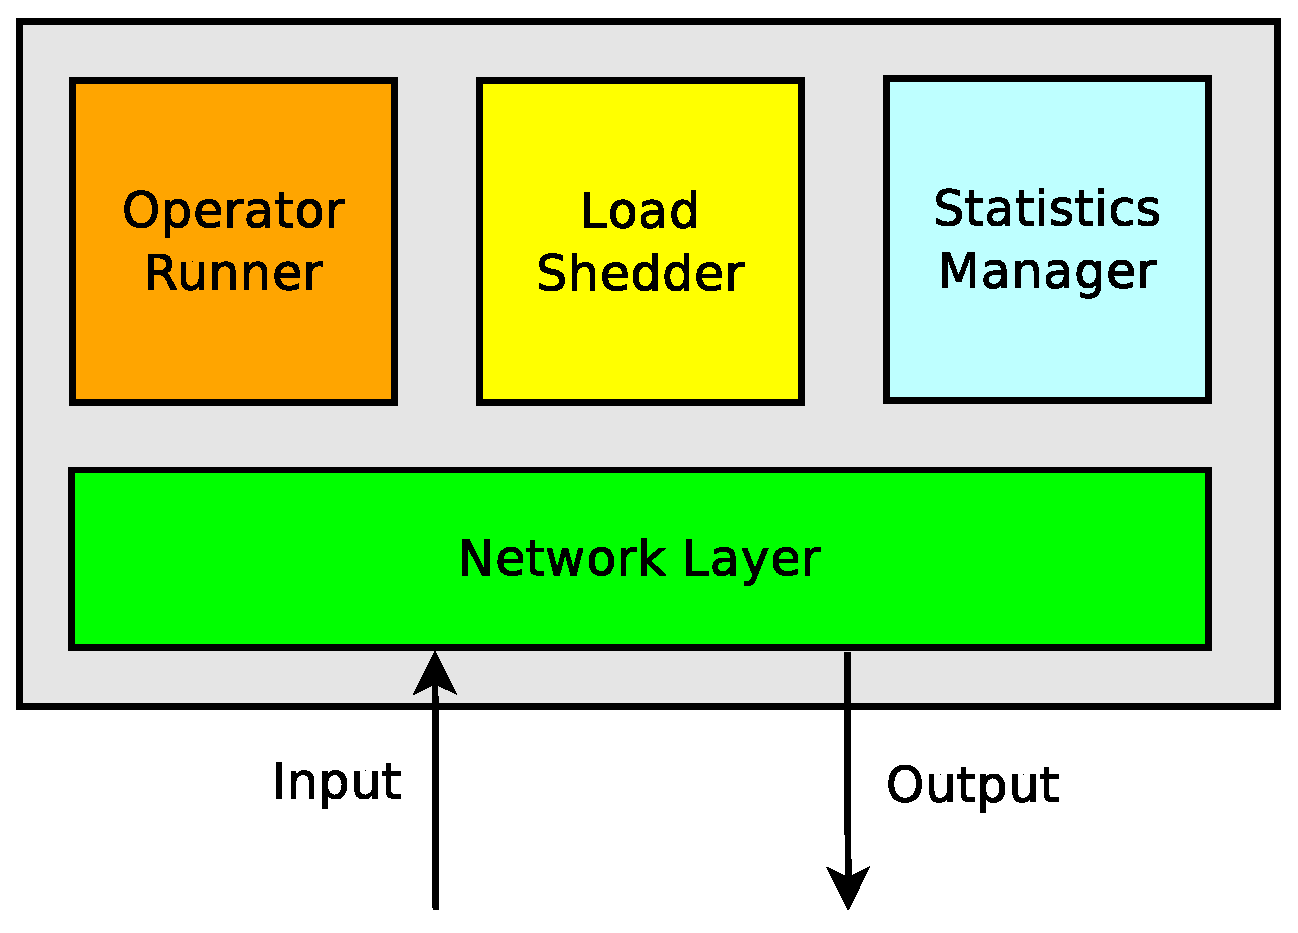
\includegraphics[width=0.5\textwidth]{img/tesi/node} 
		\caption{A high level view of a processing node, with its internal components.}
\end{figure}

\subsection*{Network Layer}  
The network layer is the component that is responsible for all the incoming and outgoing communication
of a processing node. 
It is composed of two threads: the \emph{NioConnector} thread handles all
network communication, and the \emph{RequestHandler} thread interprets the content of the received
messages and acts upon it.
We employ a many-to-one design, in which many remote connections are handled by a single pair
of receiving threads because it offers better scalability. In this way, the
number of active threads in a processing node is constant, thus avoiding the context switch overhead that
a one-to-one threading approach would have.

The \emph{NioConnector} thread acts as a receiver for remote messages as well as a sender for the
outgoing messages. All communication is done through TCP connections, which preserve the integrity of a
network message.
% Using UDP would have increased the chances of a long message being voided by the loss of one of its UDP
% chunks.
The handling of sockets is based on the Java NIO library and is completely asynchronous. This ensures a
low communication overhead and allows one thread to handle all the I/O requests. This many-to-one
design, in which one thread is responsible for all sockets, is preferable to a one-to-one approach,
with one thread for each open socket, due to its simplicity and efficiency. It only employs one CPU
core to handle network communication. Empirical evidence, based on my experience, shows that, even under heavy load and the
presence of a large number of connections, the NioConnector thread never becomes a performance
bottleneck because it only reads or writes network data.
As soon as an incoming message was fully read, it is placed in a queue of pending messages, waiting
to be interpreted by the RequestHandler thread.

The \emph{RequestHandler} thread processes incoming messages. It waits for the
NioConnector thread to place them into its queue and handles them as soon as they become available. All
inter-node communication in the system takes place through \emph{messages}. 
The chosen format for messages is UTF-8 text, with
binary chunks expressed in Base64 encoding. This simple format allows
for easy debugging, even though a binary representation would be more efficient.
The initial task performed by the RequestHandler thread is to interpret the beginning of the message to
categorise it and process it accordingly. A message can be of three kinds: it can be a message
containing \emph{tuples} to be delivered to some subquery for processing; it can contain a \emph{command
message} that triggers the execution of a remote procedure call; or it can be the request to
access the \emph{web interface}.
\vspace{-10pt}
\paragraph{Tuple Handling.}
If a message contains a tuple payload, it is directly passed to the
\emph{operator runner} component without further processing. The content of the message remains in
the network format (\ie it is passed as a string). This follows the principle of \emph{\mbox{lazy
deserialisation}}, which states that the conversion from the network format of tuples should happen as
late as possible. Tuple objects are instantiated only when they are scheduled for processing. Even their
destination (\ie the queries they belong to) is not known until then.
 
The reason for this design choice is that instantiating tuples and determining their destination is a
costly process. In particular, it may be unnecessary to perform it early, when at a later stage the whole
batch may be discarded by the \emph{load-shedder}. Delaying this operation as much as possible ensures
that no resources are wasted to instantiate and route tuples that are never processed.
Our empirical evidence suggests that an early deserialisation also poses a significant processing burden
on the RequestHandler thread, which is unable to handle all messages in a timely fashion under heavy~load.
\vspace{-10pt}
\paragraph{Command Messages.}
A message may also contain a command, triggering a corresponding remote procedure call. This can be
used for communication purposes, reporting information about the status of a node or a query to the
oracle or the query coordinator. Every node, for example, periodically reports its throughput, average
tuple latency and load information to the oracle. It also reports the achieved \sic value
for each query to the respective coordinator, which in turn calculates an aggregated value to be sent to
the oracle. 

Command messages can also be used to obtain information from another node or the oracle. For
example, when a coordinator instantiates a query, it sends a message to the oracle requesting a list
of nodes onto which to deploy the query. During the initial connection stage, when the subqueries running
on different nodes need to connect to each other, it is typical for a node to wait a certain amount
of time for the other node to be ready to accept the connection. A message is used in this situation to
probe the availability of the another node and to wait until it becomes ready.

Another use for command messages is to propagate certain values to a set of nodes. Every node, for
example, needs to be aware of the final \sic value achieved by all queries that are running on it.
By using the global \sic value achieved by every query and comparing it to the local values of the tuples
that it processes, the load-shedder can implement an intelligent load-shedding policy. Therefore, every
coordinator periodically disseminates the global \sic value of its query to all the nodes hosting subqueries.
\vspace{-10pt}
\paragraph{Web Interface.}
The RequestHandler thread is also the gateway to the node's \emph{web interface}. When receiving a
message, it checks if it is an HTTP request and, if so, it replies with a web page containing information
about the current status of the node using the information obtained from the \emph{statistics manager}.
This includes the number of hosted subqueries together with their performance as well as some global
metrics describing the status of the node, such as its average throughput and latency.
When connecting to the oracle, the web interface produces a report about the status of all processing
nodes, together with a summary of the performance achieved by all queries sorted by \sic value. The web
interface of the oracle is useful to monitor the overall performance of the system and to evaluate the
effectiveness of the shedding policy. 

\subsection*{Operator Runner}
After a batch of tuples was received, it is passed to the \emph{operator runner} for processing.
% This is the component in charge of handling the operator processing. 
The operator runner employs a fixed number of threads, each
executing a chain of operators at a time. Bounding the number of processing threads has the
advantage that tuples are processed in the order of arrival and provides more flexibility to the load
shedder, which can freeze the queue of pending jobs and analyse it to make the load-shedding decisions.

The original message, still in its network format, is encapsulated into a \emph{work unit}, a Runnable
class representing a future job to be processed. It is submitted to a ThreadPoolExecutor and placed into
a pending queue until one of the threads in the pool becomes available and executes it. The work unit
contains the logic to deserialise, route and process the tuples contained in the message that it was
assigned. The last operator of the subquery graph is a RemoteSender. It takes the result of
the subquery computation and sends it to the next processing node through the network layer. Once a work
unit has terminated its execution, it frees its execution thread so that a new work unit
can be processed.
\vspace{-10pt}
\paragraph{Thread Pool.}
At the core of the \emph{operator runner} is a \emph{thread pool}, ready to execute work units as
they are submitted. It is a subclass of ThreadPoolExecutor that augments its parent class with the
capability of stopping and resuming execution, which is needed by the load-shedder to inspect the pending
jobs queue. The number of threads is set to be equal to the number of available CPU cores. The pending
jobs queue is a list of work units. As soon as one of the threads in the pool becomes available, it
removes the oldest work unit from the queue and executes it. 

When the system is overloaded, the number of items added to the queue is
larger than the number of items removed, thus making the size of the queue grow. This increases the
latency of processing and eventually leads to an exhaustion of memory. For this reason, the thread
pool is interrupted periodically by the load-shedder, which inspects the pending batches and decides if
there is the need of discarding a certain portion of them in order to overcome overload. The choice
of which ones to discard is part of the shedding policy of the load-shedder.
\vspace{-10pt}
\paragraph{Work Unit.}
A work unit is a container class that has the blueprint to deserialise, route
and process a batch of tuples. Once a work unit is removed from the pending jobs queue and selected
for processing, it is executed by a thread from the pool. 
It starts by deserialising and instantiating the tuples contained in the message received
from the network. It then checks to which query it should be delivered. In case there are multiple
recipients, it creates a copy of itself for each query interested in its payload. After that, it calls
the \texttt{process()} function on the first operator of the query graph. This function takes the
incoming tuples and executes the operator logic, producing one or more batches as output. The work unit
passes these tuples to the next operator and continues processing until it reaches the end of the local subquery
graph. 

A work unit continues processing as long as possible instead of creating a
new work unit for each operator. This permits the system to achieve a higher throughput by reducing
overhead.
Not introducing a new work unit for each operator also guarantees that once a batch of tuples starts
processing, it is not affected by the load-shedder. An approach with one work unit per operator
may result in a batch being processed by a few operators just to be discarded by a later
execution of the load-shedder. If the subquery graph contains an operator with more than one recipient,
such as in a fan-out query, the current work unit continues processing on a single branch, while
creating a new work unit for each of the other operators. 

\subsection*{Load-Shedder}

The \emph{load-shedder} is the component that carries out the \emph{overload management} of a
processing node. When the amount of input tuples rises over a given threshold, the resources available at
the node become insufficient for processing. More tuples are given as input to the node than
what it can process, thus leading to the accumulation of jobs in the pending queue. This causes a growing
increase in latency of the tuples, until the available memory is exhausted.
\vspace{-10pt}
\paragraph{Periodic Evaluation.}
The \emph{CheckOverload} thread periodically runs and evaluates the current load situation of a node.
In the DISSP prototype, a \emph{shedding interval} of 250 milliseconds was chosen, which allows a timely
response to overcome an overload condition while keeping a low performance overhead. Every time the
CheckOverload thread executes, it calculates the number of tuples that the node is able to process
before the next load check.
If this number is greater than the number of tuples currently in the queue waiting to be processed, the
system is not overloaded and no tuples are discarded. If the number of waiting tuples is larger than the
ones that the node manages to process, a certain amount needs to be discarded. 

The system retains a record of its \emph{output rate} (\ie the amount of tuples processed within one
shedding interval). It uses this to calculate the average time needed to process a single tuple called
the \emph{tuple cost}.
Since the shedding interval is
fixed, it is possible to calculate the number of tuples that the system can process before
a new shedding iteration by dividing the \emph{shedding interval} by the \emph{tuple cost}. This
provides the number of tuples \emph{to keep}. Subtracting this number from the \emph{total number of
tuples waiting}, the system obtains the \emph{number of tuples to be discarded}.\\
These numbers depend on many factors. For example, the number of tuples received by a subquery
can be different in a given interval, or the query semantics may produce a variable load
depending on the values contained in the incoming tuples (\ie in the presence of a filter). 
Therefore, the system uses a \emph{sliding window} to average a value for the node's processing capacity
(\ie the forecast number of tuples to process in the next interval) over a few prior iterations thus
reducing the variance of these values. In summary, the periodic cycle followed by the load-shedder is as
follows:
\vspace{-10pt}
%Every time the load-shedder thread executes it follows the same processing steps:
\begin{myenumerate}
  \item Pause the thread pool
  \item Calculate the number of tuples to be discarded
  \item Choose which tuples to shed
  \item Shed the chosen tuples
  \item Resume the thread pool
  \item Update the load metrics 
\end{myenumerate}
\vspace{-10pt}
First, the thread pool has to be stopped in order to obtain the number of tuples that it contains in its
pending queue at this moment. The processing of tuples cannot happen during the execution of the
load-shedder so that it can choose what tuples to discard from a static set. 
After that, it estimates the number of tuples to be discarded, using the logic described in the previous
paragraph.
Once the number of tuples to retain is calculated, the load-shedder can make a decision about
which tuples should be discarded out of the ones available. This choice depends on the \emph{shedding
policy}. A more detailed description of different shedding policies will be given in Chapter~\ref{ch:load_shedding}. 

Then the actual tuples are discarded by removing the corresponding work units from the thread pool queue.
In the DISSP prototype, the granularity of removal is at the level of \emph{batches} because this is the
input/output unit between operators and every work unit is associated with a batch. After performing the
dropping of tuples, the thread pool is restarted and the processing of tuples continues. Before ending
its cycle, the load-shedder calculates the new updated values for the current \emph{tuple cost} and other
internal metrics. Once it finished executing, it calculates the time that it took for processing, called
the \emph{shedding time}, which it subtracts from its fixed interval of execution, called the
\emph{shedding interval}, obtaining the amount of time to sleep before its next execution.

\subsection*{Statistics Manager}
The \emph{statistics manager} is the component responsible for the calculation of the global performance
metrics of a processing node. The metrics gathered by it are used to improve the overall
performance of the system. The load-shedder can exploit its knowledge of the local utility of a
query to implement a fair shedding policy, trying to provide the same processing quality to
all the queries. The oracle, using the information about latency and throughput of nodes, can select the set of
nodes for a new deployment, trying to avoid nodes that are already heavily loaded.

The statistics manager runs periodically, by default once a minute, and calculates a number of
statistics, some of which are logged locally and some are propagated to the coordinator or the
oracle. The following is a list of the most important metrics and their function:

\textbf{Average SIC.} \emph{The average \sic value achieved by queries hosted at this node.}\\
Every subquery is aware of its global \sic value because this value is propagated from the coordinator to
all the processing nodes. This metric is sent to the oracle and can be used during the deployment of
a new query. For a fair deployment strategy, a node already hosting parts of queries
achieving a low global \sic value should not be chosen to host a new subquery. Adding further load
to the node may lead to an overload condition, thus further reducing the processing performance of the
currently running queries. 

\textbf{Average tuple drop.} \emph{The average number of tuples discarded by the node in a chosen time
interval.}\\
This value helps quantifying the amount of overload experienced by a node. It is sent to the
oracle and can be used by a deployment strategy to place a new subquery onto nodes that are not
overloaded or to avoid placing it on a node experiencing already a high tuple loss. 

\textbf{Average throughput.} \emph{The average number of tuples processed by the node in a
chosen time interval.}\\
This value can be used to quantify the spare processing capacity of a node. By
recording the value of this metric when encountering an overload condition, it is possible to have an
indication of the number of tuples per second that this node can process on average without loss. 
This value is sent to the oracle and allows a deployment strategy to choose the least loaded
nodes out of those currently not experiencing overload.\\

\textbf{Average processing latency.} \emph{The average latency in milliseconds for all the hosted
subqueries.}\\
A measure of how much time a tuple spends in this node, from when it is received to when it is delivered
to the next node. This value is sent to the oracle and can be used to discover performance bottlenecks
and to evaluate the quality of the chosen deployment strategy. 
%A good strategy would result in similar latencies at all nodes.

\textbf{Number of running subqueries.} \emph{The number of subqueries running on a node.}\\
This metric can be used to check if the deployment strategy leads to an even
deployment or to a skewed distribution of subqueries. It is sent to the oracle and can also be used to
assess the quality of the chosen deployment strategy.

\textbf{Number of connected subqueries.} \emph{The number of subqueries fully connected.}\\ 
This metric can be used to check the correct deployment of a query.
Every subquery contains at least one incoming network operator (RemoteReceiver) and one outgoing network
operator (RemoteSender). If the query deployment was successful, the number of established connections
should be equal to the number of these operators. A discrepancy indicates that one or more queries are
disconnected either temporary or permanently, which may have been caused by a network partition or a
neighbour node has crashed.


%--------------------------------------------------------------------------------------------------------

\section{Life Cycle of a Query}
\label{sec:qdep}
%  \mnote{4.4 describes the workflows in the architecture, ie how components are used to implement
% desired functionality; this is also when you introduce algorithms etc.}  \mnote{Description of the
% steps involved in the deployment of a query}
This section describes the workflow of a query, from when it is submitted to when it starts processing.
It shows how different aspects of the system are realised by describing the process of instantiating,
deploying and connecting a query.
First, a query plan is submitted in XML format. Based on this, the system creates a set of customised
operator instances. After a query has been instantiated, it is broken down into subqueries employing a
flexible partitioning policy. Each subquery is deployed on a processing node, chosen from a set of
suitable candidates provided by the oracle. Finally, the different subqueries are connected to each
other, tuples start flowing from the input providers and the processing begins.
Figure~\ref{fig:qdep} shows the steps involved in the deployment of a query.
% ----------  OVERVIEW  -----------------
\begin{myenumerate}
  \item First, the query graph is submitted in XML format. It contains the query specification
  with a list of tuples and operators to be used. It also has information about the links among
  operators. 
  \item The \emph{submitter} compiles and instantiates the XML query specification, creating the tuples
  and operator objects. Next, it starts a \emph{coordinator}, which is the entity in charge of deploying
  and monitoring the status of the query.
  \item The \emph{coordinator} creates $N$ subqueries from the original query graph according to a user
  defined partitioning policy. Next, it contacts the \emph{oracle} to obtain a set of $N$ nodes for
  deployment.\\
  \item The \emph{oracle} returns a list of the $N$ most suitable nodes available for deployment. This
  choice is dictated by a system-wide policy, such as choosing the least loaded nodes or nodes with a low
  network latency between them.
  \item Once the \emph{coordinator} receives this information, it proceeds by deploying the individual
  subqueries onto the provided \emph{processing nodes}.
  \item Each \emph{processing node} instantiates the assigned subquery and connects the query,
  establishing the required remote network connections between the operators.
  \item Finally, the \emph{input provider} operators connect to the external sources and start feeding
  tuples to the query. The query is then deployed and starts processing.
\end{myenumerate}
\begin{figure}[t!]
	\centering
	\includegraphics[width=0.6\textwidth]{img/tesi/query_deployment.eps} 
	\caption{Steps involved in the deployment of a query.}
	\label{fig:qdep}
\end{figure} 
% ---------- SUBMISSION -----------------
\subsection{Submission of Queries}
\label{sec:qsub}
%\mnote{should include ``compilation'' of tuples and ops }
The life cycle of a query begins with the submission of its query plan by a user. This is done through
the \emph{submitter} component. It interprets the XML query specification and compiles a set of custom
operator instances. Operators and tuples are compiled at run-time for better performance. The next
paragraphs introduce the concept of \emph{compiled} operators and tuples and how they are realised in the
DISSP design.
	
\subsubsection*{Compiled Operators and Tuples}
\label{sec:templates}
In the DISSP system, tuples and operators are implemented as \emph{compiled Plain Old Java
Objects (POJO)}~\cite{pojo}.
This choice was made taking performance into consideration because other options, based for example on
\emph{reflection}, are slow and can cause a potential performance bottleneck. To
instantiate a custom tuple or operator object based on the query requirements, a text \textit{template}
is completed with the information contained in the XML query specification that describes the query
producing a new Java source file, which is then compiled to bytecode by a run-time compiler.
\paragraph{XML Query Representation.} Queries are submitted to the system in an XML representation.
An XML query file contains the complete description of the query. It specifies what kind of tuples
are processed and provides a description of the \emph{tuple schemas} so that operators are aware of the
number, type and name of the fields contained in the tuples that they process. It also includes the list
of operators implementing the query semantics. Each operator is represented by an XML block, containing
its description. \\
An operator needs to be specialised before it can be used in a query. A
generic implementation is provided in a \emph{template file}, which acts as a blueprint for the operator.
It is then completed with the data included in the XML block, allowing the correct instantiation of the
operator: its \emph{name, parameters} and an indication of its \emph{subsequent operator}. An
operator either declares itself as a \emph{terminal} operator by having no subsequent operators, or as an
\emph{intermediate} operator with its output used as input to another operator.\\
Based on this information, the system reconstructs the complete query graph.
The XML query representation is used to generate a complete set of Java source files
that define the customised tuples and operators that are used in the query. These files are then compiled
and instantiated so that the query can begin processing. 

\paragraph{Templates.} Semi-complete \textrm{Java} source files represent the skeleton of a class and
are used for the efficient instantiation of customised \textit{tuples} and \textit{operators}.
All tuples share common characteristics but differ in the number of fields, their names and types. The
same is true for all operators that belong to the same type. For example, all average operators have the
same processing semantics but have different names and types of the fields to be averaged. \\
A generic blueprint for these operators comes from the generalisation of a specific instance, in which
specific names and types are replaced by textual \emph{placeholders}.
Using the information contained in the XML query description, it is possible to substitute these
placeholders with the correct details, transforming a template into a complete \textrm{Java} source file
ready for compilation.
Placeholders are all capitals keywords preceded by a dollar sign in the form ``\texttt{\$PLACEHOLDER}''.
They are replaced using the information provided in the XML file describing the query and the compiled
into actual Java objects with the required characteristics.
For this transformation, the system uses a \textit{CharSequenceCompiler}, which takes as input a string
with the content of a completed \textrm{template} file and produces an instance of a customised object.
This means that the system operates on compiled bytecode, which combines a high execution efficiency with
the flexibility of working with customised versions of tuples and operators tailored to the query
requirements.
% \lstset{ basicstyle=\ttfamily, columns=fixed, showstringspaces=false,
% commentstyle=\color{white}\upshape }  \lstdefinelanguage{XML} { morestring=[b]", %morestring=[s]{>}{<},
% morecomment=[s]{<?}{?>}, stringstyle=\color{BrickRed}, identifierstyle=\color{NavyBlue},
% keywordstyle=\color{ForestGreen}, morekeywords={type,name}% list your attributes here }
% \noindent\begin{minipage}{\textwidth} \begin{lstlisting}[language=XML,label=lst:opxml,caption=XML
% description of an Average operator] <operator name="MyAvgCpu" type="Average"> <next name="MyOutput"/>
% <parameter name="tuple"    value="simpleSchemaONE" /> <parameter name="field"    value="cpu"/>
% <parameter name="groupby"  value="idx"/> <operator> \end{lstlisting} \end{minipage} 
% \exblock{Listing~\ref{lst:opxml} shows the XML description of an \emph{Average} operator. In the first
% line the operator is characterized as being an instance of class ``Average'', described in the
% correspondant .template file, and it is given the name of ``MyAvgCpu'. Then there is the declaration of
% a \emph{next} operator, this means that this is not a terminal operator and thus its output should be
% delivered to a single local operator named ``MyOutput''. Next are 3 parameter definitions, in the form
% $\langle name, value \rangle$. The system will look for the ``\$NAME'' placeholder and will replace it
% with the string given by ``value''. Once the substitution has taken place, the .template file becomes a
% complete .java source file and is then compiled by the \emph{CharSequenceCompiler}.}
%\clearpage
% ---------------------------------
Tuples are also implemented using a template file. A parent class called \texttt{Tuple} is provided that
contains the basic processing logic common to all tuples, and every tuple class is derived from it.
In the XML query description, the user specifies a schema and a name for the tuples that are used by the
query, and the system creates a new tuple class with the required name and fields. The generic
tuple template file is then completed, substituting the placeholders with the provided data,
thus producing the Java source file of the new tuple class.

Listing~\ref{lst:tuplexml} shows the XML description of a Tuple object with three fields: a
\texttt{long} field for the timestamp named \textit{ts} and two \texttt{double} fields, one with a
numerical identifier \textit{idx} and the other for a temperature reading \textit{tmp}. These values are
inserted in the tuple template in correspondence with the ``\texttt{\$FIELD}'' placeholder, transforming
it into a complete Java source file. As a result, the compiled object contains three public fields with
the types and names from the XML listing.
 \lstset{
  basicstyle=\singlespacing\ttfamily, columns=fixed, showstringspaces=false,
  commentstyle=\color{white}\upshape }

\lstdefinelanguage{XML}
{
  morestring=[b]",
  %morestring=[s]{>}{<},
  morecomment=[s]{<?}{?>},
  stringstyle=\color{BrickRed},
  identifierstyle=\color{NavyBlue},
  keywordstyle=\color{ForestGreen}, 
  morekeywords={type,name}% list your attributes here
}
\begin{lstlisting}[language=XML,label=lst:tuplexml,caption=XML description of a Tuple]
	<schema name="simpleSchemaONE">
	    <field type="long"   name="ts"  />
	    <field type="double" name="idx" />
	    <field type="double" name="tmp" />  
	</schema>
\end{lstlisting}
 
%--------------------------------- 
Listing~\ref{lst:opxml} shows the XML description of an average operator. In the first line the
operator is defined as being an instance of class \texttt{Average}, described in the corresponding
template file, and it is given the name \texttt{MyAvgCpu}. 

Next, there is the declaration of a \textit{subsequent} operator, which means that this is not a terminal
operator. Its output should be delivered to a single local operator named \texttt{MyOutput}. 
This is followed by three parameter definitions in the form of $\langle name,
value \rangle$. The system considers the \texttt{\$NAME} placeholder and replaces it with the string
given by \texttt{value}. After this substitution, the template file becomes a
complete Java source file and is compiled by the \textit{CharSequenceCompiler}.
\lstset{
  basicstyle=\ttfamily\singlespacing,
  columns=fixed,
  showstringspaces=false,
  commentstyle=\color{white}\upshape
}

\lstdefinelanguage{XML}
{
  morestring=[b]",
  %morestring=[s]{>}{<},
  morecomment=[s]{<?}{?>},
  stringstyle=\color{BrickRed},
  identifierstyle=\color{NavyBlue},
  keywordstyle=\color{ForestGreen}, 
  morekeywords={type,name}% list your attributes here
}
\noindent\begin{minipage}{\textwidth}
\begin{lstlisting}[language=XML,label=lst:opxml,caption=XML description of an Average operator]
	<operator name="MyAvgCpu" type="Average">
	    <next name="MyOutput"/>
	    <parameter name="tuple"    value="simpleSchemaONE" />
	    <parameter name="field"    value="cpu"/>
	    <parameter name="groupby"  value="idx"/>
	<operator>
\end{lstlisting}
\end{minipage}	
\clearpage
The DISSP system provides a number of general-purpose operator templates: \textit{window operators}
provide transformations over windows, holding the input of an operator until a certain condition is
reached; \textit{I/O operators} act as gateways to the system and provide the conversion from
external to a system tuple representation (and vice versa); \textit{network operators} support
inter-node communication so that a query can be partitioned and distributed across several nodes;
and \textit{\mbox{data manipulation operators}} are used to process the data and are equivalent to the
\textit{relation-to-relation} operators in CQL.

% ---------- PARTITIONING -----------------
\subsection{Partitioning of Queries}
\label{sec:qpart}
After a query was instantiated based on its XML representation, it is broken down into chunks called
\emph{subqueries}. These are computationally less intensive than the complete query and can be deployed
across a set of \emph{processing nodes}. The partitioning process can follow different strategies. 
This section presents two policies: one that takes into account the processing
\emph{load} of the newly created partitions and another that multiplexes particularly heavy
partitions over several nodes, executing them in parallel according to a horizontal partitioning
approach.
\vspace{-10pt}
\paragraph*{Load-Aware Partitioning.}
%\todo{figure load-aware}  
The partitioning of a query graph can follow a strategy that groups operators with similar processing
loads.
Such a \emph{load-aware} strategy tries to obtain subqueries with similar costs in order to spread evenly
the processing load. It is similar to the one described in \cite{borealis-load}.
Since the query partitioning occurs before the query is deployed, the system estimates the cost of an
operator based on its expected \emph{input rate} and \emph{load coefficient}.\\
The expected input rate is calculated for an operator by analysing its direct predecessors in the query
graph and their window operators. The estimate can be more precise in the case of \emph{aggregate
operators}, such as average, because they produce a single output every time that they are triggered. For
\emph{filters}, the estimate is more difficult and must take their selectivity into account. \\ 
The load coefficient of an operator has to be determined offline and estimates the computational
complexity of the operator. A synthetic load of fixed size is input to the operator on a testbed machine
and its CPU load is measured. \\
By multiplying the input rate and the load coefficient, it is possible to
estimate the future load of an operator. The initial partitioning can then divide the query graph
evenly. Note that this should only be thought of as a starting point to be augmented with the run-time
migration of operators or subqueries. This accounts for inaccuracies in the initial estimates. 
\vspace{-10pt}
\paragraph*{Horizontal Partitioning}

The cost of a query is not only determined by the number of operators that it employs. Even queries with
a simple query graph can be computationally expensive due to a high rate of incoming tuples or
the complexity of an operator. In such cases, the partitioning of the query it is not limited to
the grouping of operators into subqueries but includes the rewriting of the query graph. The costly
operator, or subquery, is decomposed so that multiple copies of it can run in parallel on several
processing nodes.
The original input data is split by a \emph{router} operator that sends the chunks in turn to the nodes
hosting the decomposed operator copies.
This approach performs a horizontal scale out of the operator. The output of these operator copies is
sent to a collector operator, which finalises the processing to achieve the original semantics of the
unpartitioned operator.

For example, a costly \emph{average} operator could be decomposed into three copies, each
calculating the average for a $1/3$ of the input. The final average is then calculated by the collector
based on the partial averages.
Other operators, such as \emph{filter}, do not need a further collector phase, and only take a union of
the partial results to generate the final output. 

\begin{figure}[t!]
	\centering	
	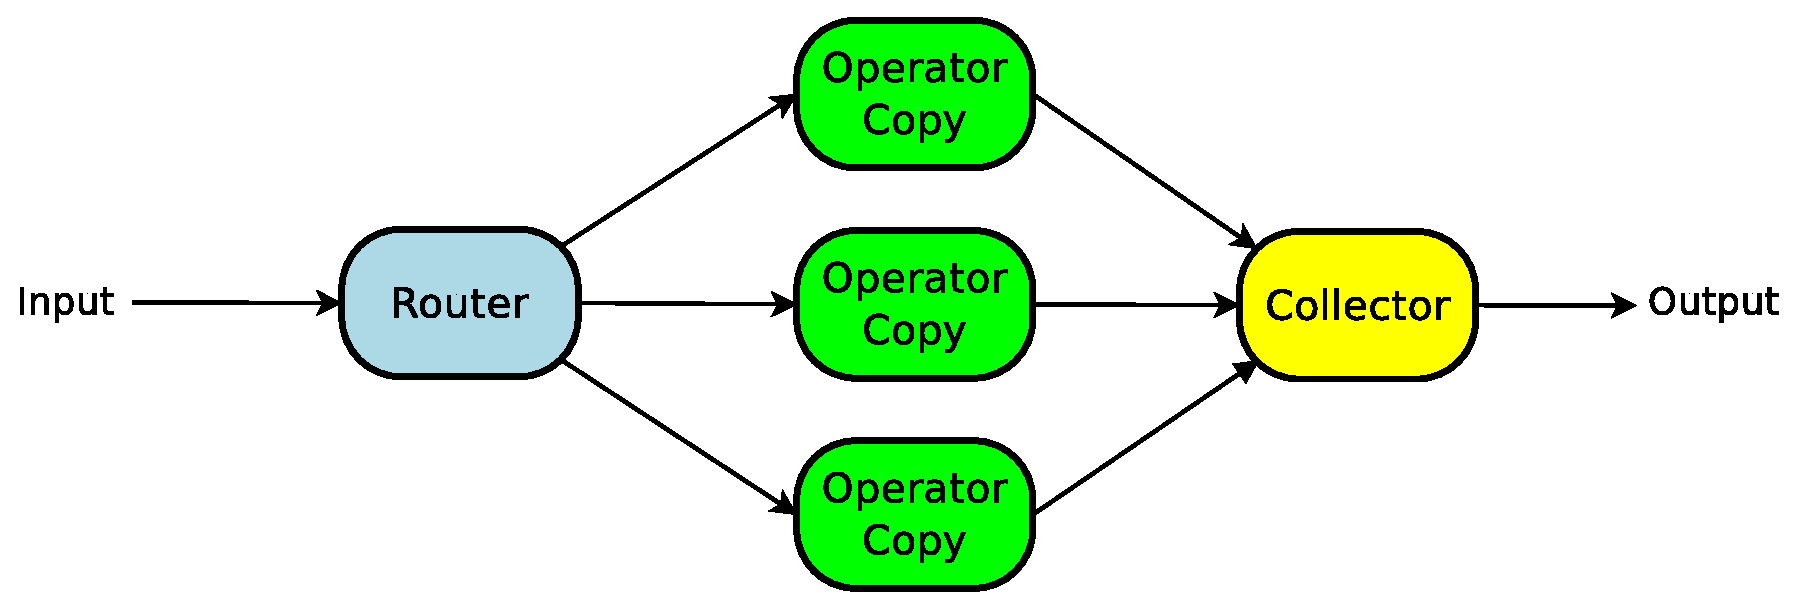
\includegraphics[width=0.8\textwidth]{img/tesi/map-reduce2}
	\caption{Horizontal partitioning of an operator. }
	\label{fig:mr-part}
\end{figure}

Figure~\ref{fig:mr-part} shows the modified query graph of a query rewritten using the
horizontal partitioning strategy. The original query with one expensive operator is transformed so that
three copies of the operators run on different processing nodes. A round-robin router operator evenly
splits the incoming tuples among them. A final replica of the operator, an aggregate in this case,
collects the partial results and outputs the final value. 
\begin{comment}	


% ---------- DEPLOYMENT -----------------
\subsection{Deployment of Queries}

After being partitioned into subqueries, a query is ready to be deployed. 



% ---------- CONNECTION -----------------
\subsection{Connection of Queries}
\label{sec:qsub}
	
\mnote{should include connection and start up of queries}

\begin{figure}
	\centering	
	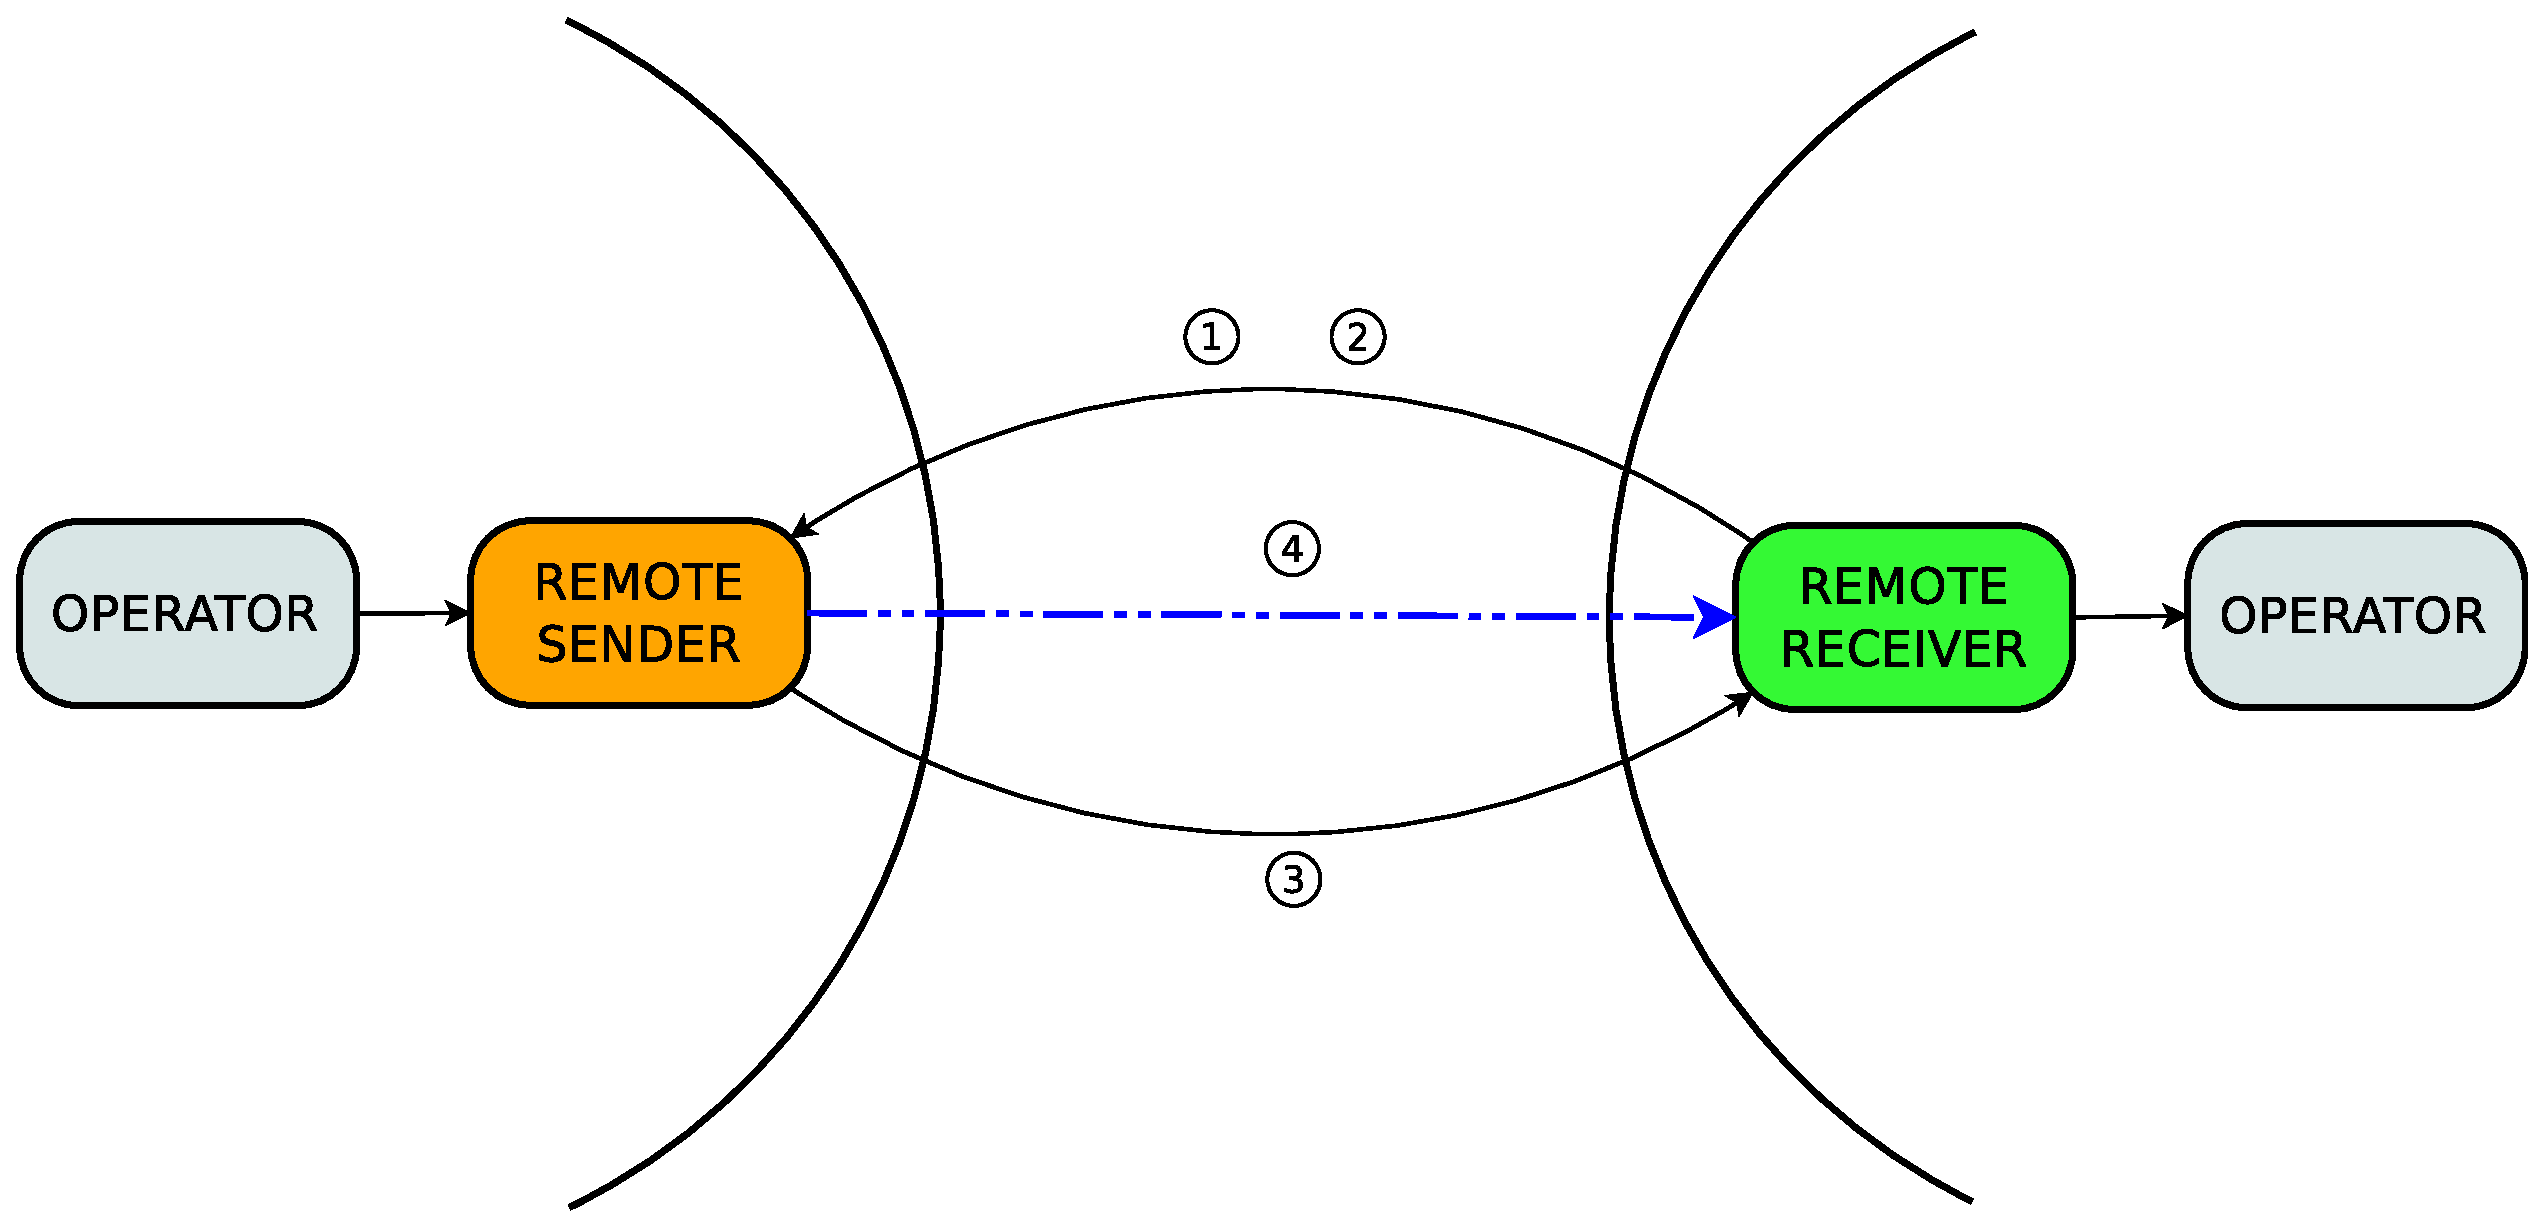
\includegraphics[width=0.8\textwidth]{img/tesi/remote_connection.eps}
	\caption{Remote connection of 2 operators}
	\label{fig:remconn}
\end{figure}
	
\end{comment}




%--------------------------------------------------------------------------------------------------------

\section{Summary}
This chapter presented the design of the DISSP prototype system, a stream processing engine designed to
realise the quality-centric data model described in Chapter~\ref{ch:data_model}.
First, it presented the goals that drove the design of the system, such as the ability to perform
efficient processing under overload, the embedded calculation of the \sic metric and the support for
adapting the \mbox{load-shedding} policy according to user needs.
It explained how the theoretical concepts presented in the description of the data model
can be implemented in the basic components of a stream processing system.

The chapter then described the \emph{system-level components}, in particular their roles
and their interactions. In every DISSP deployment, queries run on one or more \emph{processing
nodes}. These process tuples provided by a set of \emph{input providers} that
convert external inputs to an appropriate system format. New queries are introduced into the system by a
\emph{submitter}. For each query a \emph{coordinator} is spawned that is in charge of its deployment
and management. An \emph{oracle} oversees the processing of all queries, gathering information about
their performance and providing a global view of the system.

After looking at the system as a whole, the focus shifted to the internal components of processing
nodes. Every node exchanges command messages and tuples with other nodes and the oracle through a
\emph{network layer}. An \emph{operator runner} routes tuples to the assigned subqueries
and manages their processing through the graph of operators. A \emph{load-shedder}
overcomes overload by selecting tuples to be discarded, while a \emph{statistic manager} keeps
track of important metrics about the performance of a node.

The chapter ended with the description of the deployment of a query. It used this workflow to
describe the detailed steps involved from the submission of a query to when it
starts processing.
It explained how tuples and operators are compiled at run-time from an XML query description, and how
the original query graph is partitioned into subqueries to be deployed on multiple processing nodes.

The next chapter focuses on the load-shedding process in more detail, presenting a \emph{fair
shedding} algorithm that exploits the \sic metric to allocate resources among queries evenly. 
The goal is for them to all achieve the same performance in terms of the quality of the computed results.

	



		

